\documentclass[
  %fleqn,     das ist für die zentrierung
	parskip=half,
	captions=tableheading,
  titlepage=firstiscover, 		%************************************************** by Rk
	bibliography=totoc		%*************************************by Rk
	]{scrartcl}			
% \usepackage{etex}
% \reserveinserts{28}

%Das ist für die Kopfzeile
\usepackage[headsepline]{scrlayer-scrpage}
\pagestyle{scrheadings}
\clearpairofpagestyles
\ofoot{\pagemark}
\ohead{\headmark}
\automark{section}

% Warnung, falls nochmal kompiliert werden muss		%*************************************by Rk
\usepackage[aux]{rerunfilecheck}

% unverzichtbare Mathe-Befehle
\usepackage{amsmath}
% viele Mathe-Symbole
\usepackage{amssymb}
% Erweiterungen für amsmath
\usepackage{mathtools}
\usepackage{upgreek}
% Fonteinstellungen
\usepackage{fontspec}				%************************************************** by Rk
% Latin Modern Fonts werden automatisch geladen
% Latin Modern Fonts werden automatisch geladen
% Alternativ zum Beispiel:
%\setromanfont{Libertinus Serif}
%\setsansfont{Libertinus Sans}
%\setmonofont{Libertinus Mono}

\usepackage{polyglossia}
\usepackage[				%************************************************** by Rk
	backend=biber,
]{biblatex}  	
%Quellendatenbank	
\setmainlanguage{german}			
\addbibresource{lit.bib}		%************************************************** by Rk


\usepackage{expl3}
\usepackage{xparse}

\usepackage{physics}

\usepackage[unicode, german]{hyperref}
\usepackage[autostyle]{csquotes}
\usepackage[
  math-style=ISO,    % ┐
  bold-style=ISO,    % │
  sans-style=italic, % │ ISO-Standard folgen
  nabla=upright,     % │
  partial=upright,   % ┘
  warnings-off={           % ┐
    mathtools-colon,       % │ unnötige Warnungen ausschalten
    mathtools-overbracket, % │
  },                       % ┘
]{unicode-math}

% traditionelle Fonts für Mathematik
\setmathfont{Latin Modern Math}
% Alternativ zum Beispiel:
%\setmathfont{Libertinus Math}

\setmathfont{XITS Math}[range={scr, bfscr}]
\setmathfont{XITS Math}[range={cal, bfcal}, StylisticSet=1]

% Zahlen und Einheiten
\usepackage[
  locale=DE,                 % deutsche Einstellungen
  separate-uncertainty=true, % immer Fehler mit \pm
  per-mode=symbol-or-fraction,       % ^-1 für inverse Einheiten
  % output-decimal-marker=.,   % . statt , für Dezimalzahlen
]{siunitx}

% chemische Formeln
\usepackage[
  version=4,
  math-greek=default, % ┐ mit unicode-math zusammenarbeiten
  text-greek=default, % ┘
]{mhchem}

% Wenn man andere Schriftarten gesetzt hat,
% sollte man das Seiten-Layout neu berechnen lassen
\recalctypearea{}				%************************************************** by Rk


% richtige Anführungszeichen 
\usepackage[autostyle]{csquotes}

% schöne Brüche im Text
\usepackage{xfrac}

% Grafiken können eingebunden werden
\usepackage{graphicx}
% größere Variation von Dateinamen möglich
% \usepackage{grffile}
\usepackage{scrhack}

% Verbesserungen am Schriftbild
\usepackage{microtype}

% Standardplatzierung für Floats einstellen
\usepackage{float}
\usepackage[section, below]{placeins}
% \usepackage[..]{caption}
\floatplacement{figure}{htbp}
\floatplacement{table}{htbp}

\usepackage{booktabs}
\usepackage{subcaption}
% \usepackage{subfig}
\author{%
  Raphael Rico Kaiser\\%
  \href{raphael.kaiser@tu-dortmund.de}{raphael.kaiser@tu-dortmund.de}%
  \texorpdfstring{\and}{,}%
  Hendrik Trojan\\%
  \href{hendrik.trojan@tu-dortmund.de}{hendrik.trojan@tu-dortmund.de}%
}

\publishers{TU Dortmund - Fakultät Physik}
\usepackage{romannum}
\AtBeginDocument{\pagenumbering{arabic}}

\NewDocumentCommand \e {}
{
  \symup{e}
}

\NewDocumentCommand \const {}
{
  \text{const.}
}

\NewDocumentCommand \fig {mmm}
{
\begin{figure}
    \centering 
    \includegraphics[width=9cm]{#1}
    \caption{#3}
    \label{#2}
   \end{figure}
\nocite{*}
}

\usepackage{romannum}
\usepackage{listings}
\lstset{numbers=left, numberstyle=\tiny, numbersep=5pt}
\lstset{language=Perl}
\AtBeginDocument{\pagenumbering{arabic}}

% \title{
\includegraphics[scale=0.8]{../logo.jpg} \\ \vspace*{1cm} V14 \\ - Gammatomographie -}
\title{
\includegraphics[scale=0.8]{../logo.jpg} \\ \vspace*{1cm} V44 \\ - Röntgenreflektometrie -}

%\title{test}
\date{Durchführung: 05.11.2021, Abgabe: XX.11.2021}

\begin{document}

\maketitle

\tableofcontents
\newpage

\section{Ziel}
In diesem Versuch soll ein beschichteter Siliziumwafer mittels Röntgenreflektometrie untersucht werden. Es sollen die Dichte, Rauigkeit und Schichtdicke des Films mittels Intensitätsmessungen bestimmt werden. %Oder was anderes? Rauigkeit von der Grenzfläche?

\section{Theorie}
\label{sec:theorie}

\subsection{Grundlagen der Röntgenreflexivität} %Titel ändern
Röntgenstrahlen sind elektromagnetische Wellen im Wellenlängenbereich von etwa $\SI{5}{\pico\meter}$ bis $\SI{10}{\nano\meter}$.
Trifft eine solche Welle auf ein Medium mit Brechungsindex $n_2$, wird diese zum Teil reflektiert und zum Teil transmittiert und gebrochen. Das ist schematisch in \ref{fig:Brechungsindex} zu sehen. 
Der komplexe Brechungsindex berücksichtigt sowohl die Brechung als auch die Dämpfung durch Absorption und ist durch den folgenden Ausdruck definiert
\begin{equation}
    n = 1 - \delta + i \beta,
\end{equation}
wobei $\beta$ die Absorption und $\delta$ eine Korrektur beschreibt.
Für Röntgenstrahlen ist der Realteil des Brechungsindex kleiner als 1, wodurch die Möglichkeit zur Totalreflexion besteht.
Aus dem Snelliusschen Brechungsgesetz
\begin{equation}
    n_1 \cos(\alpha_i) = n_2 \cos(\alpha_f)
\end{equation}
und der Tatsache, dass $Re(n_2) < 1$ folgt, dass bei dem kritischen Winkel $\alpha_c$ die transmittierte Welle in einem Winkel von $\SI{0}{\degree}$ zur Grenzfläche steht und somit bei Winkeln unterhalb des kritischen Winkels Totalreflexion entsteht, d.h. es gibt keine transmittierte Welle. Dieser kritische Winkel wird näherungsweise beschrieben durch
\begin{equation}
    \alpha_c \approx \sqrt{2 \, \delta} \approx \lambda \, \sqrt{\frac{r_e \, \rho}{\pi}},
\end{equation}
wobei $r_e$ der Elektronenradius und $\rho$ die Elektronendichte des Materials ist.

\begin{figure}
    \centering
    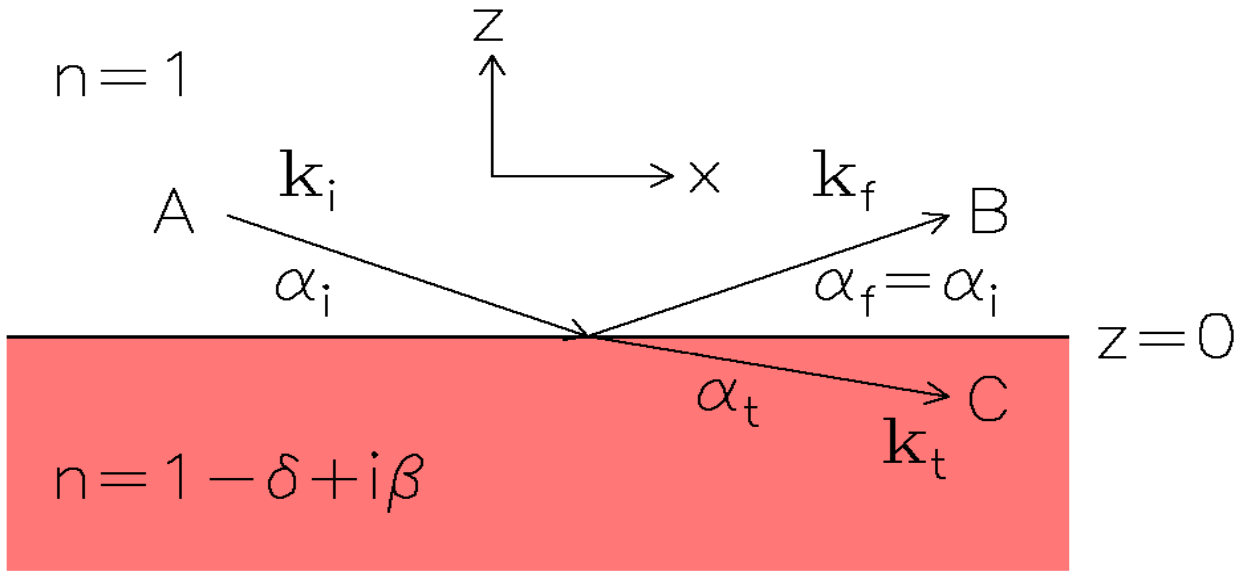
\includegraphics[width=0.7\linewidth]{./figures/Brechungsindex.png}
    \caption{.}
    \label{fig:Brechungsindex}
\end{figure}

%neues Unterkapitel?
Die Fresnelschen Formeln beschreiben quantitativ die Reflexion und Transmission einer ebenen elektromagnetischen Welle an einer ebenen Grenzfläche. %Formeln auch hinschreiben oder unnötig?
Im Fall von Röntgenstrahlung muss nicht zwischen parallel und senkrecht polarisierter Strahlung unterschieden werden und die Fresnelkoeffizienten lauten somit
\begin{equation}
    r = \frac{n_1 \, \cos(\alpha_1) \, - \, n_2 \, \cos(\alpha_2)}{n_1 \, \cos(\alpha_1) \, + \, n_2 \, \cos(\alpha_2)},
\end{equation}

\begin{equation*}
    t = \frac{2 \, n_1 \, \cos(\alpha_1)}{n_1 \, \cos(\alpha_1) \, + \, n_2 \, \cos(\alpha_2)}.
\end{equation*}


\subsection{Mehrschichtsysteme}
Bei einem aus mehreren Schichten bestehenden System wird die einfallende Strahlung sowohl an der Oberfläche, als auch an den Grenzflächen der einzelnen Schichten reflektiert. Das ist schematisch in \ref{fig:Kiessig} dargestellt.
Durch die konstruktive und destruktive Interferenz der reflektierten Strahlen entstehen Oszillationen in der detektierten Intensität. Diese sogenannten Kiessig-Oszillationen sind abhängig vom Schichtabstand $d$, weshalb dieser mithilfe der Lage der Minima in der Reflexionskurve bestimmt werden kann durch
\begin{equation}
    d = \frac{\lambda}{2 \, \Delta \alpha_i}.
\end{equation}
Dabei ist $\lambda$ die Wellenlänge und $\Delta \alpha_i$ die Differenz der Einfallswinkel an den einzelnen Schichten.
Ein Beispiel einer solchen Reflexionskurve ist in \ref{fig:Kurve} zu sehen.

\begin{figure}
    \centering
    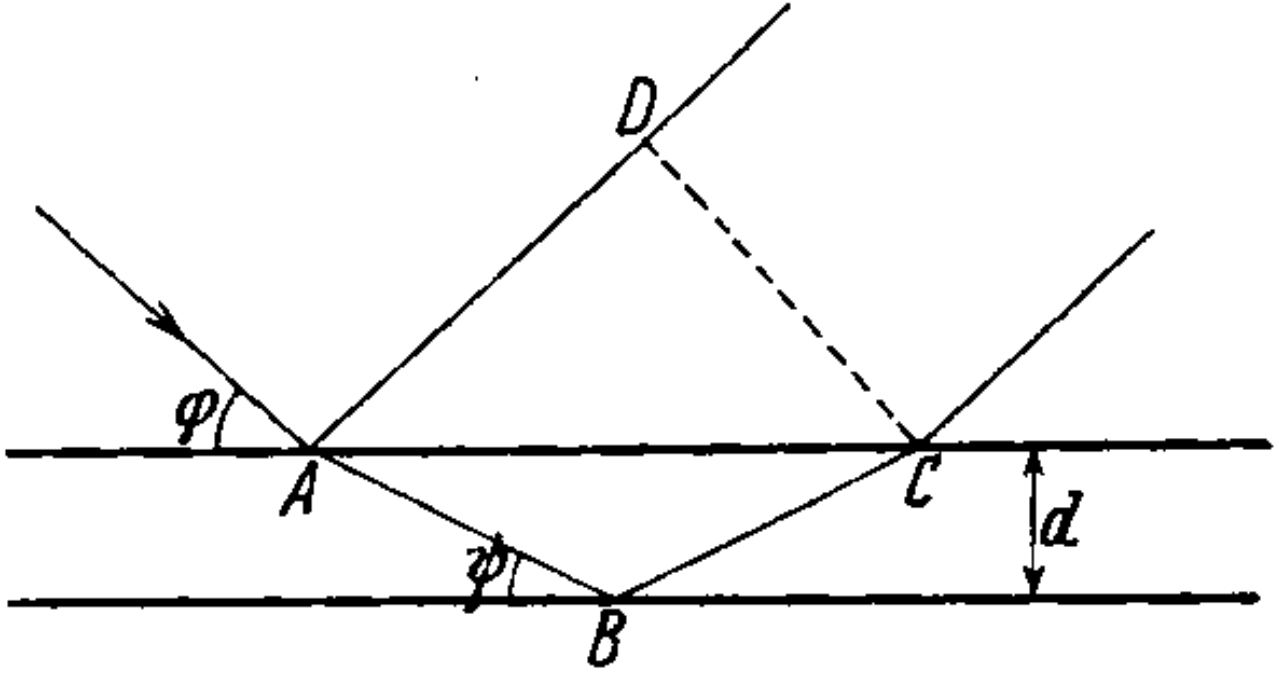
\includegraphics[width=0.5\linewidth]{./figures/Kiessig.png}
    \caption{...}
    \label{fig:Kiessig}
\end{figure}

\begin{figure}
    \centering
    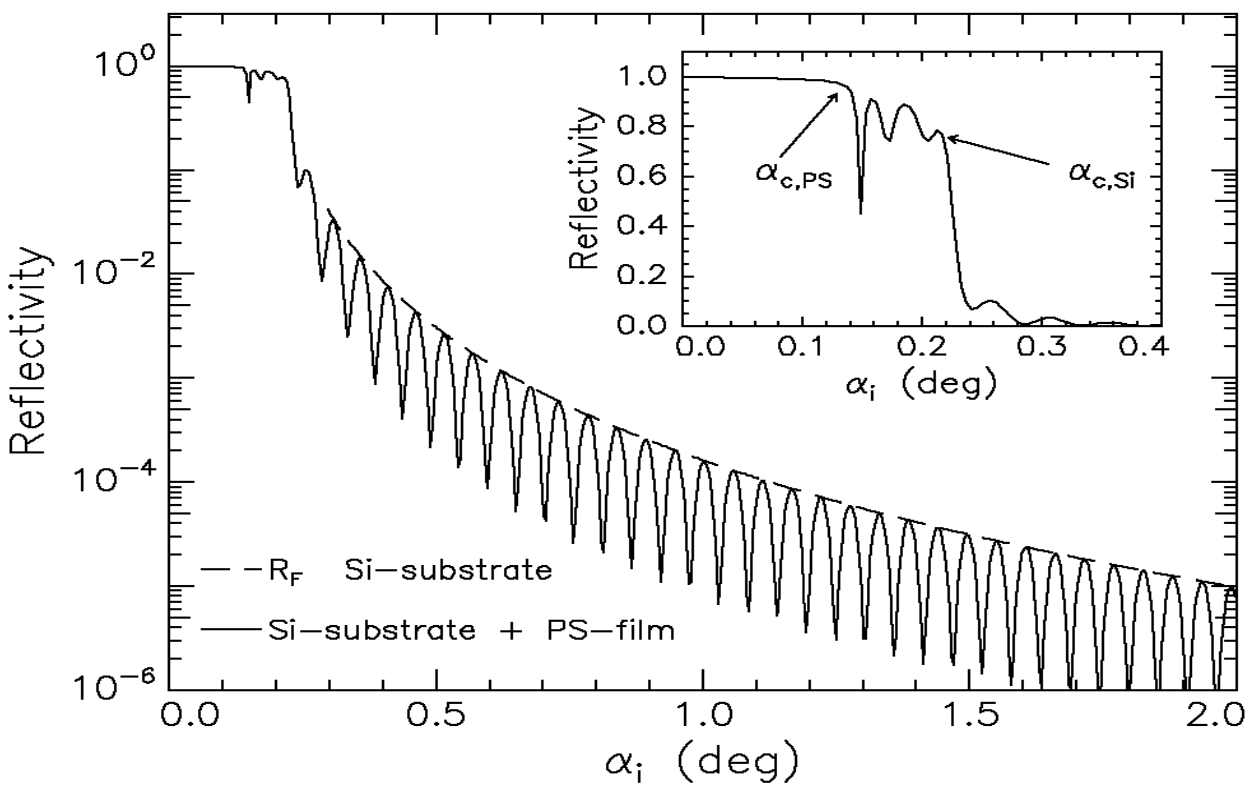
\includegraphics[width=0.7\linewidth]{./figures/Kurve.png}
    \caption{...}
    \label{fig:Kurve}
\end{figure}

Haben die Schichten unterschiedliche Brechungsindizes, ist die Reflektivität komplizierter. Um die Reflektivität eines solchen Systems zu berechnen, wird der Parratt-Algorithmus verwendet.
Dieser berechnet rekursiv das Verhältnis der reflektierten und transmittierten Wellen an der i-ten Grenzfläche
\begin{equation}
    X_i = \frac{R_i}{T_i} = \exp(-2 \, i \, k_{z,i} \, z_i) \frac{r_{i, i+1} \, + \, X_{i+1} \, \exp(2 \, i \, k_{z,i+1} \, z_i)}{1 \, + \, r_{i,i+1} \, X_{i+1} \, \exp(2 \, i \, k_{z,i+1} \, z_i)}.
\end{equation}
Die Fresnelreflektivität der i-ten Grenzfläche $r_{i, i+1} = \frac{k_{z,i} - k_{z,i+1}}{k_{z,i} + k_{z,i+1}}$ wird aus der z-Komponente des Wellenvektors $k_{z,i} = k \sqrt{n^2_i - \cos^2(\alpha_i)}$ berechnet.

Das System besteht aus $N$ Grenzflächen. Dabei bildet das Substrat die unterste Schicht, welche als unendlich dick angenommen wird.
Ein Mehrschichtsystem mit unterschiedlichen Brechungsindizes ist in \ref{fig:Mehrschicht} skizziert.

\begin{figure}
    \centering
    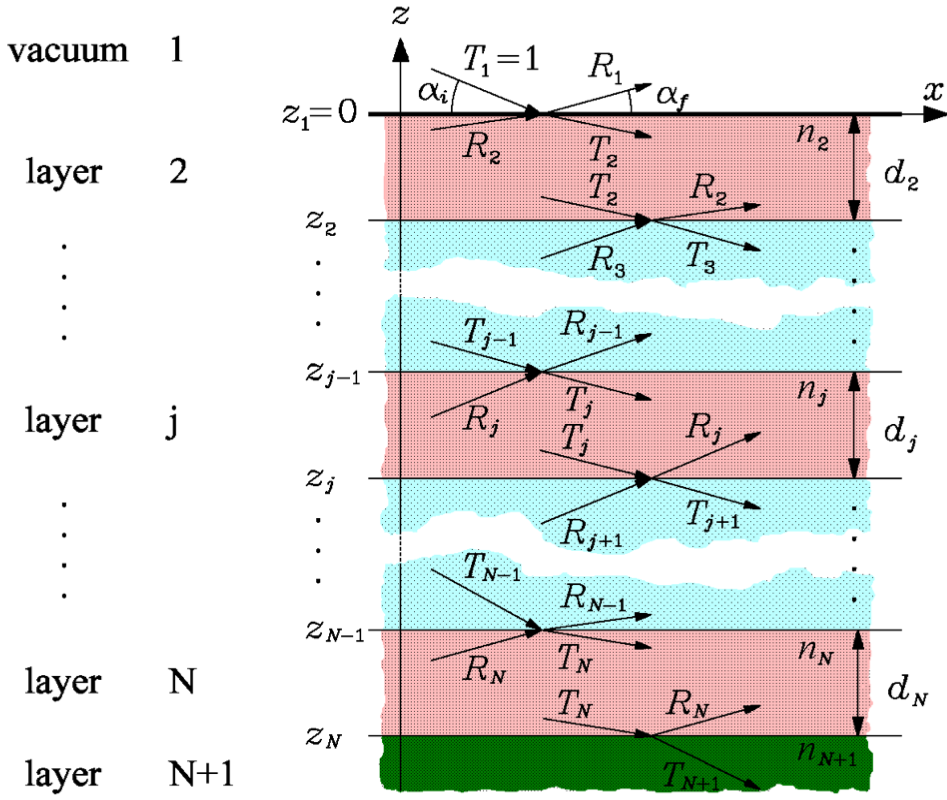
\includegraphics[width=0.7\linewidth]{./figures/Mehrschicht.png}
    \caption{.}
    \label{fig:Mehrschicht}
\end{figure}



\subsection{Raue Oberflächen}
Da reale Oberflächen eine Rauigkeit in Form von mikroskopischen Unebenheiten aufweisen und nicht glatt sind, müssen die Fresnelkoeffizienten modifiziert werden. Die reflektierte Intensität einer rauen Grenzfläche ist geringer als die einer glatten. Im Paratt-Algorithmus werden die Fresnelkoeffizienten durch die modifizierten Fresnelkomponenten ersetzt, um die Reflektivität eines Mehrschichtsystems mit rauen Grenzflächen zu bestimmen. Diese modifizierten Fresnelkoeffizienten werden folgendermaßen berechnet
\begin{equation}
    \tilde{r}_{i,i+1} = r_{i,i+1} \, \exp(-2 \, k_{z,i} \, k_{z,i+1} \, \sigma^2_i),
\end{equation}

\begin{equation}
    \tilde{t}_{i,i+1} = t_{i,i+1} \, \exp((k_{z,i} \, - \, k_{z,i+1})^2) \sigma^2_i / 2.
\end{equation}
%"root-mean-square" Rauigkeit sigma erklären



\subsection{Geometriefaktor und Geometriewinkel}
Bei kleinen Einfallswinkeln trifft der Strahl eine größere Fläche als die Probenoberfläche, wodurch nicht die gesamte eingestrahlte Intensität reflektiert und detektiert wird (siehe \ref{fig:Geometriewinkel}).
Erst wenn der Einfallswinkel, oder Geometriewinkel, genügend groß ist, trifft der gesamte Strahl auf die Oberfläche und wird reflektiert.
Um die Reflektivität zu korrigieren, wird der Geometriefaktor
\begin{equation}
    G = \frac{D \, \sin(\alpha_i)}{d_0}
\end{equation}
genutzt, wobei $D$ der Durchmesser der Probenoberfläche, $\alpha_i$ der Einfallswinkel und $d_0$ die Strahlbreite ist.
Für Einfallswinkel, die mindestens so groß wie der Geometriewinkel sind, beträgt der Geometriefaktor $G = 1$. 

\begin{figure}
    \centering
    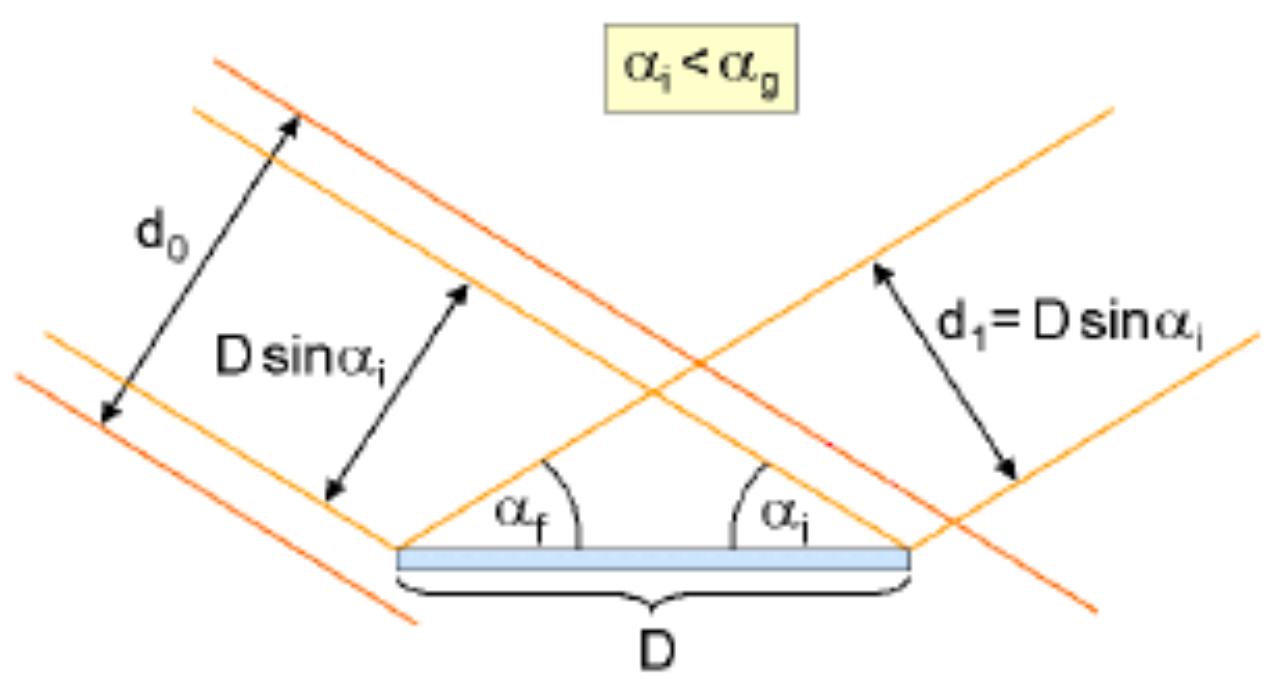
\includegraphics[width=0.7\linewidth]{./figures/Geometriewinkel.png}
    \caption{Schematische Darstellung des auf die Probe treffenden Strahls und des Gesamtstrahls. \cite{anleitung}} %Zitat?
    \label{fig:Geometriewinkel}
\end{figure}



\section{Durchführung}
\label{sec:durchfuehrung}

Der Versuch wird an einem D8-Labordiffraktometer (siehe \ref{fig:D8}) durchgeführt.
Dabei wird eine Probe von einer Röntgenröhre, die mit einer Spannung von $\SI{40}{\kilo\volt}$ und einem Strom von $\SI{35}{\milli\ampere}$ betrieben wird, bestrahlt und die reflektierte Strahlung trifft auf einen Detektor. %umformulieren
Die Probe ist ein mit einem Polymerfilm beschichteter Siliziumwafer, welcher als Substrat dient.
Vor der Messung muss die Probe im Aufbau mittels mehrerer Scans justiert werden.

\begin{figure}
    \centering
    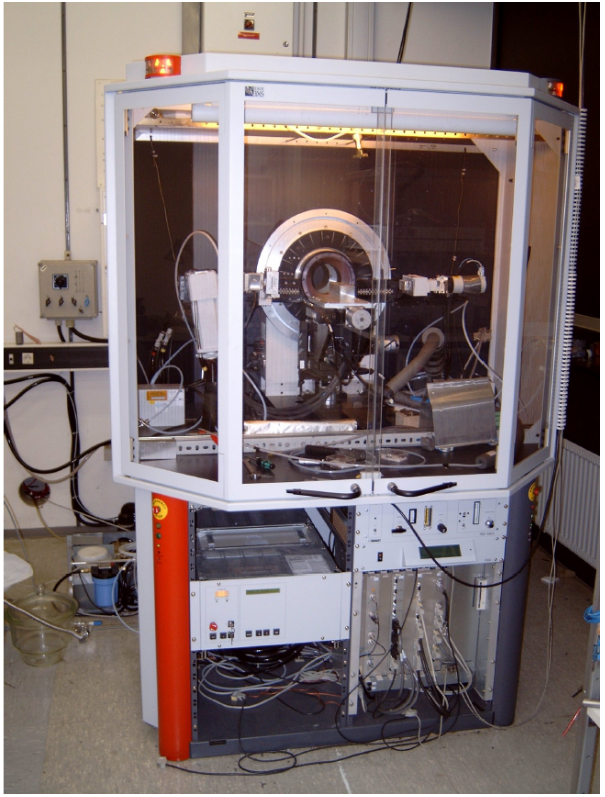
\includegraphics[width=0.5\linewidth]{./figures/D8.png}
    \caption{D8-Labordiffraktometer. \cite{anleitung}}
    \label{fig:D8}
\end{figure}



\subsection{Justage}
\textbf{Detektorscan}
\newline
Zunächst wird die Probe aus dem Strahl gefahren und die Röntgenröhre auf $\SI{0}{\degree}$ bewegt. Der Detektor wird beim Detektorscan um einen kleinen Winkelbereich um die Röhre bewegt. Dabei ergibt die aufgenommene Intensität eine Gaußverteilung. Das Maximum dieser Verteilung ist die neue Nullposition des Detektors.

\textbf{Z-Scan}
\newline
Anschließend wird die Probe im Strahl positioniert. Beim Z-Scan wird die Probe in der Höhe verschoben. Die Intensität nimmt immer weiter ab, je weiter die Probe in den Strahl fährt. Die neue z-Position der Probe ist dort, wo die halbe maximale Intensität detektiert wird, da die Probe den Strahl halb abschatten soll.

\textbf{Rockingscan}
\newline
Da der Strahl eventuell noch nicht parallel zur Probenoberfläche verläuft, wird ein Rockingscan durchgeführt. Dieser dreht die Röntgenröhre und den Detektor mit konstanter Winkelsumme um die Probe. Das entspricht einer Drehung der Probe im Strahl. Das Ziel dieses Scans ist es, die Probe in den Drehpunkt des Labordiffraktometers zu bringen und die Winkeleichung der Röhre in Bezug auf die Probe zu verbessern.
%Muss man auch sagen wie?

%\textbf{Zweiter Z-Scan}
Nach den drei Scans wird erneut der Z-Scan durchgeführt, damit die Probe wieder den Strahl halb abschattet.
%\textbf{Zweiter Rockingscan}
Ein zweiter Rockingscan wird unter einem Winkel durchgeführt, um die Probe noch exakter zu justieren.
%\textbf{Dritter Z-Scan}
Der letzte Z-Scan wird ebenfalls unter diesem Winkel durchgeführt und gewährleistet die endgültige halbe Abschattung. %umformulieren?



\subsection{Messung}
Die eigentliche Messung besteht aus einem Reflektivitätsscan und einem diffusen Scan.

Beim Reflektivitätsscan sind der Röhren- und Detektorwinkel gleich groß. Es wird in einem Bereich von $\SI{0}{\degree}$ bis $\SI{2.5}{\degree}$ mit einer Schrittweite von $\SI{0.005}{\degree}$ und einer Messzeit von $\SI{5}{\second}$ gemessen.

Bei dem diffusen Scan ist der Detektorwinkel um $\SI{0.1}{\degree}$ gegenüber dem Röhrenwinkel verschoben. Ansonsten wird die selbe Messung wiederholt. Dieser Scan ist wichtig, um die wahre Reflektivität zu erhalten. %wieso?


\section{Auswertung}
\subsection{Justierung und Kalibrierung}
Bevor die eigentlichen Messergebnisse ausgewertet werden, finden eine Reihe von Kalibrationsmessungen statt,
welche den Zweck erfüllen die Röntgenröhre optimal zu justieren und Zwischenergebnisse zu liefern.
Diese Kalibrationsmessungen werden im folgenden zuerst behandelt und ausgewertet.

\subsection{Der Detektorscan}

Die erste Messung ist die des Detektorscans welcher in \autoref{fig:detec} dargestellt ist. 
In diesem Plot ist die Detektorintensität in Abhängigkeit des Einfallwinkels zu sehen. 
Die Messung wurde über eine Bereich von $ -0,3° \text{ bis } 0,3° $ durchgeführt.
Die Messwerte wurden anschließend an einen Gausfit mit der Formel 
\begin{equation*}
    I(\alpha) = \frac{a}{\sigma\sqrt{2\pi}} \exp\left( \frac{-\left( \alpha - \alpha_0\right)^2}{2 \sigma} \right)
\end{equation*}
angepasst.
Die Fitparameter sind 
\begin{align*}
    a &= 107447.10 \pm 759.63 \\
    \alpha_{0} &= \SI{0.0107 \pm 0.0003}{\degree} \\
    \sigma &=  0.045 \pm 0.00037
\end{align*} 
Anhand des Graphen lässt sich die Halbwertsbreite sowie die maximale Detektorintensität ermitteln.
Die Halbwertsbreite beträgt $\text{FWHM} = 0.102°$ und die maximale Intensität $I_\text{max}=107447.10 \pm 759.63$.
\begin{figure}
    \centering
    \includegraphics[width=11cm]{build/detector_scan.pdf}
\end{figure}
\FloatBarrier

\subsection{Der Z-Scan}

Mit Hilfe des Z-Scans lässt sich die Strahlenbreite der Röntgenröhre näherungsweise bestimmen.
Dazu werden die abfallende und ansteigende Flanke des Scans betrachtet. 
Der Z-Scan ist in \autoref{fig:z} zu sehen.
\begin{figure}
    \centering
    \includegraphics[width=11cm]{build/z_scan.pdf}
    \caption{Verlauf des Z-Scans. Anhand der z-Achse lässt sich die Position der Probe im Strahlengang der Röntgenröhre identifizieren. 
            Mit fallendem z-Wert wird die Probe immer weiter in der Strahlengang geschoben. Der grüne Kasten markiert die Strahlenbreite. 
            Die Strahlbreite beträgt $\SI{0,3}{\milli\meter}$. }
    \label{fig:z}
\end{figure}
\FloatBarrier
Die ermittelte Strahlbreite beträgt
\begin{equation*}
    d =\SI{0,3}{\milli\meter}. 
\end{equation*}
Aus der Strahlbreite und der Probendicke $D = \SI{20}{\milli\meter}$ lässt sich der Geometriewinkel errechnen.
\begin{align*}
    \alpha_g &= \arcsin(\frac{d}{D})\\
    \alpha_g &= \SI{0.86}{\degree}.
\end{align*}

\subsection{Der Rockingscan}

Anhand des Rockingscans \autoref{fig:dreieck} lässt sich der Geometriewinkel durch ablesen bestimmen.
Der Geometriewinkel beträgt
\begin{align*}
    \alpha_1 &= \SI{-0.76}{\degree}\\    
    \alpha_2 &= \SI{0.68}{\degree}\\    
    \alpha_g &= \frac{|\alpha_1|+|\alpha_2|}{2}\\
    \alpha_g &= \SI{0.72}{\degree}.    
\end{align*}
\begin{figure}
    \centering
    \includegraphics[width=11cm]{build/dreieck.pdf}
    \caption{Verlauf des Rockingscans. Der Rockingscan liefert durch ablesen einen Geometriewinkel von $\alpha_g = \SI{0.72}{\degree}$.}
    \label{fig:dreieck}
\end{figure}

\subsection{Der Reflektivitätsscans und die Dispersionsprofile}
In \autoref{fig:alles} ist die Reflektivität in Abhängigkeit des Einfallwinkels dargestellt.
Dazu wurde die Reflektivität auf das 5 fache der Intensität normiert, da die Messdauer nach den Kalibrationsmessung 5 mal so lang gewesen ist. 

Bei Auswertung der Hauptmessung werden zu Beginn die Messwerte (schwarzer Graph, \autoref{fig:alles}) um die Messwerte des
diffusen Scans (roter Graph) korrigiert. Die Messwerte des diffusen Scans werden von Messwerten abgezogen um auftretende Rückstreueffekte zu 
eliminieren. Der entstandene Graph (orange) in ebenfalls in \autoref{fig:alles} zu sehen. 

Anschließend wird mit Hilfe der \autoref{eq:TODO} der Geometriefaktor berechnet und der zuvor korrigierte Graph um den Geometriefaktor korrigiert. 
Die Korrektur um den Geometriefaktor geschieht, da bei geringen Einfallwinkeln nicht die vollständige Intensität auf die Probenoberfläche trifft. 
Dieser Graph ist in \autoref{fig:alles} dunkelblau dargestellt. 
Werden die Kiesing Oszillationen betrachtet und die Positionen der Minima eingezeichnet, lässt sich mit der \autoref{eq:TODO} die 
Schichtdicke von Polystyrol berechnen.
Die ermittelte Schichtdicke ist
\begin{align*}
    d_\text{ps} = \SI{890}{\angstrom}.
\end{align*}
\begin{figure}
    \centering
    \includegraphics[width=12cm]{build/messwerte_relativ.pdf}
    \caption{Reflektivitätsscans und Dispersionsprofile. Farblich dargestellt sind die unterschiedlichen Graphen und kritischen Winkel.
            Der hellblaue und der lilafarbene Graph sind mit dem Parratt-Algorithmus entstanden und repräsentieren eine glatte und eine raue Oberfläche der Probe. }
    \label{fig:alles}
\end{figure}
\FloatBarrier
Mit Hilfe des Parratt-Algorithmus lässt sich ebenfalls die Schichtdicke bestimmen. 
Dazu werden die unterschiedlichen Parameter siehe \autoref{eq:params} in den Parrat-Algorithmus \autoref{eq:TODO} eingesetzt.
\begin{equation}\label{eq:params}    
    \begin{split}
        \lambda &= \SI{855}{\angstrom}\\
        \delta_\text{ps} &= 0,6\cdot 10^{-6}\\
        \delta_\text{si}&= 6,8\cdot 10^{-6} \\
        n_\text{luft} &= 1 \\
        n_\text{ps} &= 1 - \delta_\text{ps} \\
        n_\text{si} &= 1 - \delta_\text{ps} 
    \end{split}
\end{equation}
Die Parameter werden durch geringe Änderungen variiert bis die entstandene hellblaue Kurve siehe \autoref{fig:alles} mit der gemessenen
Kurve näherungsweise übereinstimmt. 
Der Parratt-Algorithmus mit diesen Parametern repräsentiert eine glatte Oberfläche.

Werden die Rauigkeiten $\sigma_\text{ps} = 7,9\cdot 10^{-10}$ und $\sigma_\text{si} = 5,7\cdot 10^{-10}$
betrachtet ergibt sich der lilafarbene Plot in \autoref{fig:alles}.

Mit Hilfe der unterschiedlichen Dispersionen von Polystyrol und Silizium lassen sich die kritischen Winkel ausrechnen,
dazu wird \autoref{eq:TODO} verwendet.
Die kritischen Winkel sind
\begin{align*}
    \alpha_\text{c,ps}& = \SI{0,063}{\degree}\\
    \alpha_\text{c,si}& = \SI{0.211}{\degree}.
\end{align*}
Diese Winkel sind ebenfalls in \autoref{fig:alles} eingezeichnet.

\section{Diskussion}
Der durch die Probendicke und die Strahlbreite ermittelte Geometriewinkel $\alpha_\text{g} =0,85°$ weicht um 15\%
von der Geometriewinkel der mit am Graphen des Rockingscans $\alpha_\text{g} =0,72°$ abgelesen wurde ab. 
Diese Abweichung ist damit zu erklären, dass die Strahlbreite anhand des Z-Scans bestimmt worden ist und die Strahlbreite
ebenfalls durch ablesen am Graphen fehlerbehaftet ist.

Wird der Graph der Messwerte und die der beiden mit dem Parratt-Algorithmus erstellen Graphen miteinander verglichen, so lässt sich 
erkennen das diese gut übereinstimmen.
Die Schichtdicken betragen
\begin{align*}
    d_\text{ps} &= \SI{855}{\angstrom}\\
    d_\text{parrat} &= \SI{890,25}{\angstrom}.
\end{align*}
Aus den Schichtdicken ergibt sich eine Abweichung von 3,96\%.

Die ermittelten Dispersionen und die Literaturwerte\cite{V44old} sind
\begin{align}
    \begin{split}    
        \delta_\text{ps} &= 0,6\cdot 10^{-6}\\
        \delta_\text{si}&= 6,8\cdot 10^{-6} \\
        \delta_\text{ps,lit} &= 3,5\cdot 10^{-6}\\
        \delta_\text{si,lit}&= 7,6\cdot 10^{-6}
    \end{split} 
\end{align}
Es fällt auf die Dispersion von Polystyrol deutlich mehr von Literaturwert abweicht als die von Silizium.
Die Abweichungen betragen bei Polystyrol 82,86\% und bei Silizium 10,53\%.
Die geringe gemessene Dispersion von Polystyrol ist darauf zurückzuführen, dass die Kiesig-Oszillationen eine
sehr geringe Amplitude gezeigt haben.

Die ermittelten kritischen Winkel anhand des Parratt-Algorithmus und die Literaturwerte\cite{V44old} sind
\begin{align*}
    \alpha_\text{c,ps} &= \SI{0.063}{\degree} \\
    \alpha_\text{c,ps,lit} &= \SI{0.153}{\degree} \\
    \alpha_\text{c,si} &= \SI{0.211}{\degree} \\
    \alpha_\text{c,si,lit} &= \SI{0.210}{\degree}.
\end{align*}
Es fällt auf das der kritische Winkel von Silizium passt sehr gut zu dem Literaturwert passt.
Bei dem Winkel von Polystyrol ist allerdings eine große Abweichung zu erkennen.
Diese ist aber darauf zurückzuführen das sich der kritische Winkel aus der zuvor bestimmten Dispersion errechnet
und diese ebenfalls stark abweicht. 

\section{Programmcode Parratt-Algorithmus}
\begin{lstlisting}{Name}
    #Versuchsgrößen
 l = 1.54e-10 # Wellenlänge
 ai = np.arange(0, 2.5+0.005, 0.005)
 #print(ai)
 k = 2*np.pi / l #Wellenvektor
 qz = 2*k * np.sin(ai) #Wellenvektorübertrag -> y-Werte der Theoriekurve
 
 #Parameter des Parratt-Algorithmus
 
 #Dispersionen   #die werte orientieren sich an den theoriewerten
                 #with with the wave of my finger an the flick of my dick
 #d1 = 0.7e-6 #Polysterol Disperion
 #d2 = 6.7e-6 #Silizium 
 d1 = 0.6e-6 #Polysterol Disperion
 d2 = 6.8e-6 #Silizium 
 
 #Brechungsindizes
 n1 = 1 #Luft
 n2 = 1 - d1 #Polysterol
 n3 = 1 - d2 #Silizium
 
 #Rauigkeit
 s1 = 7.9e-10 #Polysterol 
 s2 = 5.7e-10 #Silizium 
 z = 855e-10 
 ########################################################################################################
 # Parratt
 
 def parratt(z):
     kz1 = k * np.sqrt(np.abs(n1**2 - np.cos((np.pi/180) * ai)**2))
     kz2 = k * np.sqrt(np.abs(n2**2 - np.cos((np.pi/180) * ai)**2))
     kz3 = k * np.sqrt(np.abs(n3**2 - np.cos((np.pi/180) * ai)**2))
     #
     r12 = (kz1 - kz2) / (kz1 + kz2) * np.exp(-2 * kz1 * kz2 * s1**2)
     r23 = (kz2 - kz3) / (kz2 + kz3) * np.exp(-2 * kz2 * kz3 * s2**2)
     #
     x2 = np.exp(0 - (kz2 * z) * 2j) * r23
     x1 = (r12 + x2) / (1 + r12 * x2)
     par = np.abs(x1)**2
 
     return par
 
 
 plt.plot(ai[42:],parratt(z)[42:],'-')#Parrat (glattes Si)') Werte rausgenommen damit die oszillationen am anfang verschwinden
 
 ########################################################################################################
 
 def parratt2(z):
     kz1 = k * np.sqrt(np.abs(n1**2 - np.cos((np.pi/180) *ai)**2))
     kz2 = k * np.sqrt(np.abs(n2**2 - np.cos((np.pi/180) *ai)**2))
     kz3 = k * np.sqrt(np.abs(n3**2 - np.cos((np.pi/180) *ai)**2))
     #
     r12 = (kz1 - kz2) / (kz1 + kz2)
     r23 = (kz2 - kz3) / (kz2 + kz3)
     r13 = ((kz1 - kz3) / (kz1 + kz3))**2
     #
     x2 = np.exp(0 - (kz2 * z) * 2j) * r23
     x1 = (r12 + x2) / (1 + r12 * x2)
     par = np.abs(x1)**2
     
     return par
 
 plt.plot(ai[42:],parratt2(z)[42:],'-',color= 'purple')# Parrat (raues Si) 
 ########################################################################################################
 
 # kritische Winkel Ablesen
 alpha_crit_ps= 0.054          # Polystyrol (abgelesen)
 plt.axvline( x = alpha_crit_ps,linewidth = 0.9,linestyle= '--',color ='k', label = r'$\alpha_c$ für PS (gemessen)')
 print('\n')
 print('Der abgelesene kritische Winkel für Polystyrol beträgt',alpha_crit_ps,'°.\n')
 
 alpha_crit_si=  0.195          # Silizium (abgelesen)
 plt.axvline( x = alpha_crit_si,linewidth = 0.9,linestyle= '--',color ='purple', label = r'$\alpha_c$ für Si (gemessen)')
 print('Der abgelesene kritische Winkel für Silizium  beträgt',alpha_crit_si,'°.\n')
 
 # Theoriewerte Literatur
 alpha_crit_ps_theo= 0.153   # Polystyrol
 plt.axvline( x = alpha_crit_ps_theo,linewidth = 0.9,linestyle= '--',color = 'brown', label = r'$\alpha_c$ für PS (Theorie)')
 print('Der Literaturwert für den kritischen Winkel von Polystyrol beträgt',alpha_crit_ps_theo,'°.\n')
 
 #alpha_crit_si_theo= 0.223   # Silizium
 alpha_crit_si_theo= 0.21   # Silizium cheat mode on sei neuer Theoriewert 
 plt.axvline( x = alpha_crit_si_theo,linewidth = 0.9,linestyle= '--',color = 'pink', label = r'$\alpha_c$ für Si (Theorie)')
 print('Der Literaturwert für den kritischen Winkel von Silizium beträgt',alpha_crit_si_theo,'°.\n')
 
 #parrat line angepasst
 plt.axhline( y = 0.7 ,xmin = 0.096,xmax = 0.193 ,linewidth = 1.2,linestyle= '-') #parratt plateo
 
 plt.legend(loc="best")
 
 # kritischer Winkel Rechnung
 alpha_crit_si_rech = np.degrees(np.arccos(1-d2))
 alpha_crit_ps_rech = np.degrees(np.arccos(1-d1))
 
 
 print('Der errechnete kritische Winkel von Polystyrol anhand des Parrart Algorithmus ist:\n ',alpha_crit_ps_rech,'°.\n' )
 print('Der errechnete kritische Winkel von Silizium anhand des Parrart Algorithmus ist:\n ',alpha_crit_si_rech,'°.\n' )
 
 ########################################################################################################
 plt.savefig("build/messwerte_relativ.pdf")
 ########################################################################################################
 
\end{lstlisting}
 
\nocite{*}
\printbibliography{}
\end{document}